\chapter{遅延聴覚フィードバックが身体運動に与える影響の調査}
本章では,第4章で開発されたシステムと第6章で決定された実験条件を用いて,遅延聴覚フィードバックが身体運動に及ぼす影響を若年者及び高齢者に対して調査した結果について述べる.「高齢者は若年者に比べて聴覚フィードバックの遅延に対する許容度が高い」という仮説は,4の倍数に達したときにのみ遅延を発生させるシステムを用いて検証する.第6章の予備実験により,4の倍数に達する直前の押下間隔と4の倍数に達した直後の押下間隔の差の二乗の平均値及び中央値が遅延時間の増加に比例して増大すること,及び4の倍数に達したときの遅延が全体のボタン押下間隔のばらつきを拡大させるという可能性が示唆された.これらの予備実験で得られた考察を基に,仮説の検証を行う.
\section{調査方法}
若年者及び高齢者を対象に行ったボタン押し課題による遅延聴覚フィードバックが身体運動に与える影響の調査の方法を以下に示す.
\begin{enumerate}
  \item 被験者に図4.1のシステムを用意する.
  \item 4章の手順1から手順2までに述べた方法によって,ボタン押し課題を実施する.
  \item ヘッドホンから出力される音遅延時間をランダムに変更して実験者がアプリケーション上で指定した回数だけ手順2を繰り返す.このとき,実験者が提示する回数は,7.2節で提示する遅延時間の種類である.
\end{enumerate}
また,得られた結果は,遅延時間に応じて各被験者の観測値の四分位範囲(IQR)と第一・第三四分位数を算出し,外れ値を除外するために第一四分位数-1.5×IQR以下と第三四分位数+1.5×IQR以上の値を排除して分析した.
\section{調査条件及び調査対象}
\begin{table}[hbtp]
  \caption{若年者の実験Aにおける遅延時間の提示順}
  \label{table:young_a}
  \centering
  \begin{tabular}{lccc}
    \hline
    提示順 & 遅延時間 & 被験者数 & 年齢\\
     & [ms] & & [平均 $\pm$ 標準偏差]\\
    \hline \hline
    提示順1  & 10, 30, 110, 10, 70, 90, 50  & 8 & 22.1 $\pm$ 0.78\\
    提示順2  & 10, 70, 30, 110, 50, 90, 10  & 8 & 22.4 $\pm$ 0.99\\
    提示順3  & 10, 110, 90, 50, 10, 30, 70  & 8 & 22.3 $\pm$ 1.09\\
    提示順4  & 10, 50, 90, 10, 30, 70, 110  & 7 & 22.7 $\pm$ 0.88\\
    提示順5  & 10, 30, 10, 50, 110, 70, 90  & 7 & 23.1 $\pm$ 0.64
\\
    \hline
  \end{tabular}
\end{table}
\begin{table}[hbtp]
  \caption{若年者の実験Bにおける遅延時間の提示順}
  \label{table:young_b}
  \centering
  \begin{tabular}{lccc}
    \hline
    提示順 & 遅延時間 & 被験者数 & 年齢\\
     & [ms] & & [平均 $\pm$ 標準偏差]\\
    \hline \hline
    提示順1  & 10, 25, 35, 30, 40, 20, 10, 15  & 7 & 22.6 $\pm$ 1.29\\
    提示順2  & 10, 15, 40, 10, 35, 25, 30, 20  & 7 & 22.9 $\pm$ 1.25\\
    提示順3  & 10, 30, 25, 10, 40, 20, 35, 15  & 7 & 23.6 $\pm$ 1.18\\
    提示順4  & 10, 30, 20, 10, 15, 35, 25, 40  & 7 & 22.1 $\pm$ 1.36\\
    提示順5  & 10, 40, 10, 25, 30, 20, 15, 35  & 6 & 23.5 $\pm$ 0.76
\\
    \hline
  \end{tabular}
\end{table}
\begin{table}[hbtp]
  \caption{高齢者の実験Aにおける遅延時間の提示順}
  \label{table:old_a}
  \centering
  \begin{tabular}{lccc}
    \hline
    提示順 & 遅延時間 & 被験者数 & 年齢\\
     & [ms] & & [平均 $\pm$ 標準偏差]\\
    \hline \hline
    提示順1  & 10, 30, 110, 10, 70, 90, 50  & 8 & 63.5 $\pm$ 3.94\\
    提示順2  & 10, 70, 30, 110, 50, 90, 10  & 8 & 70.1 $\pm$ 4.96\\
    提示順3  & 10, 110, 90, 50, 10, 30, 70  & 8 & 68.4 $\pm$ 4.50\\
    提示順4  & 10, 50, 90, 10, 30, 70, 110  & 9 & 70.2 $\pm$ 6.48\\
    提示順5  & 10, 30, 10, 50, 110, 70, 90  & 8 & 75.5 $\pm$ 4.72
\\
    \hline
  \end{tabular}
\end{table}
\begin{table}[hbtp]
  \caption{高齢者の実験Bにおける遅延時間の提示順}
  \label{table:old_b}
  \centering
  \begin{tabular}{lccc}
    \hline
    提示順 & 遅延時間 & 被験者数 & 年齢\\
     & [ms] & & [平均 $\pm$ 標準偏差]\\
    \hline \hline
    提示順1  & 10, 30, 110, 10, 70, 90, 50  & 4 & 22.5 $\pm$ 0.88\\
    提示順2  & 10, 70, 30, 110, 50, 90, 10  & 3 & 22.0 $\pm$ 0.0\\
    提示順3  & 10, 110, 90, 50, 10, 30, 70  & 3 & 23.7 $\pm$ 1.3\\
    提示順4  & 10, 50, 90, 10, 30, 70, 110  & 3 & 21.7 $\pm$ 0.49\\
    提示順5  & 10, 30, 10, 50, 110, 70, 90  & 3 & 22.7 $\pm$ 1.8
\\
    \hline
  \end{tabular}
\end{table}
\newpage
\section{調査結果}
\subsection{外れ値の除去}
データの代表的な統計量,特に平均や標準偏差は,対象のデータ分布が正規分布に従っている場合にその真の特性を正確に反映する.したがって,遅延時間ごとに得られたボタンの押下時間間隔のデータが正規分布に従うかどうかを確認することが必要である.これにより,分散や標準偏差を用いてデータ分布のばらつきを評価することの妥当性を検討する.帰無仮説を「ボタン押下時間間隔のデータの母集団の分布は,正規分布に従う」として,コルモゴロフ・スミルノフ検定を用いて,有意水準5%で観測値が正規分布に従うかどうかを検定する.遅延時間に応じたボタンの押下時間間隔のデータのヒストグラムを図7.1,図7.2,図7.3,図7.4に示す.また,正規性の検定の結果を表7.1に記載する.
外れ値の除去は,被験者ごとに各遅延時間での観測値を
\begin{figure}[bt]
  \centering
  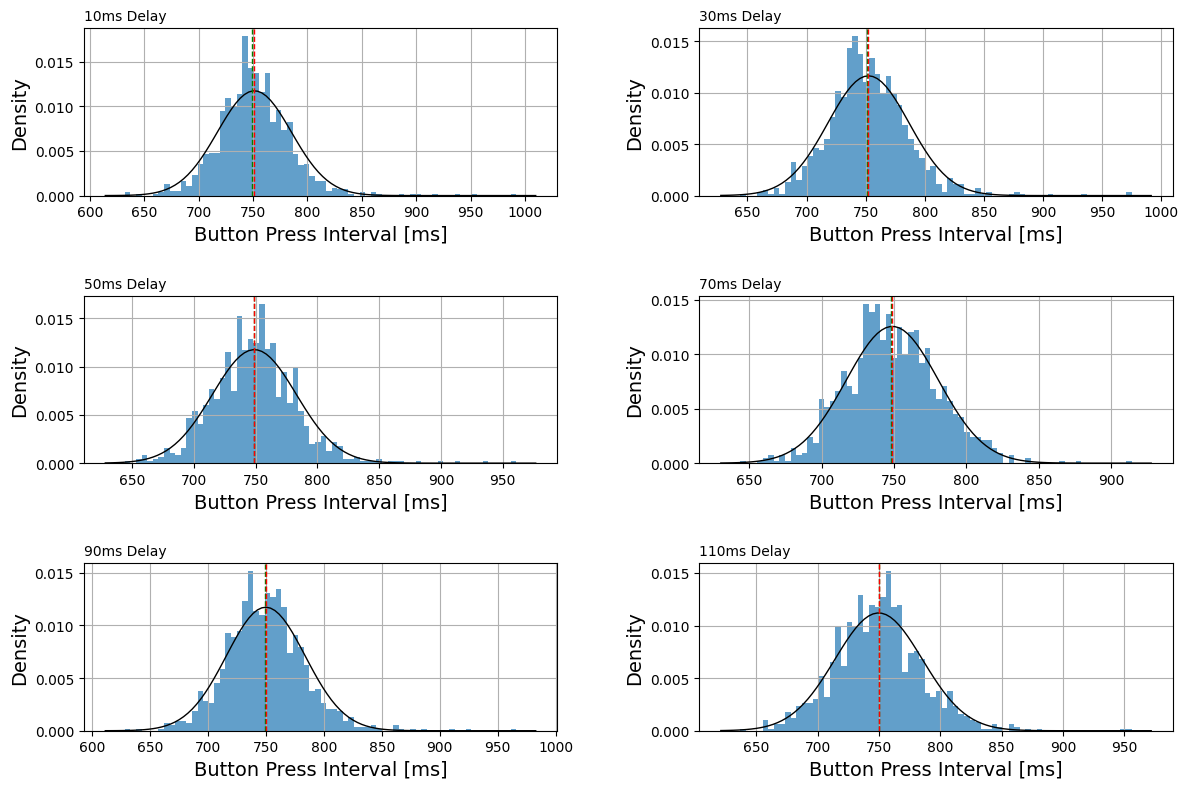
\includegraphics[scale=0.4]{figures/Production/110ms_Distribution_of_observations.png}
  \caption{実験Aにおける遅延時間ごとの若年者のデータの分布}
\end{figure}
\subsection{遅延時間と評価指標の関係}
\begin{figure}[bt]
  \centering
  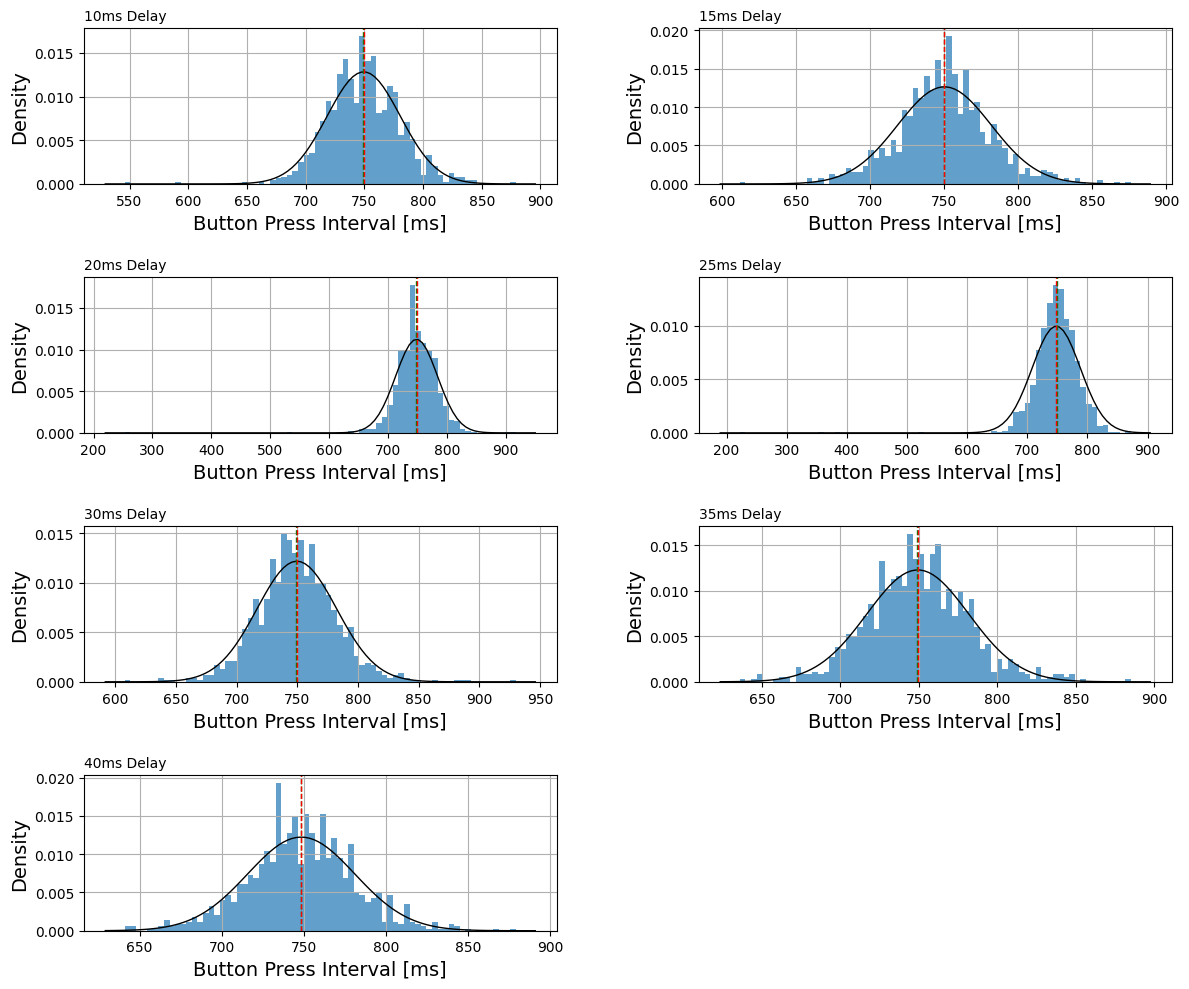
\includegraphics[scale=0.4]{figures/Production/40msDistribution_of_observations.png}
  \caption{実験Bにおける遅延時間ごとの若年者のデータの分布}
\end{figure}

